\documentclass{article}

% Appearance
%--------------------------------------
\usepackage[a4paper,width=170mm,top=18mm,bottom=22mm,includeheadfoot,marginparsep=2cm]{geometry}
\usepackage{url}
%--------------------------------------

% Colors
%--------------------------------------
\usepackage{color}
\definecolor{lightyellow}{rgb}{1,0.98,0.9}
\pagecolor{lightyellow}
%--------------------------------------

% Language
%--------------------------------------
\usepackage[utf8]{inputenc}
\usepackage[T2A]{fontenc}
\usepackage{hyphenat}
%--------------------------------------

% References
%--------------------------------------
\usepackage{biblatex}
\addbibresource{biblio.bib}
%--------------------------------------

% Footnotes
%--------------------------------------
\usepackage[hang]{footmisc}
\setlength{\footnotemargin}{14pt}
\setlength{\skip\footins}{20pt}
%--------------------------------------

% Columns
%--------------------------------------
\usepackage{multicol}
\setlength{\columnsep}{24pt}
%--------------------------------------

% Graphics
%--------------------------------------
\usepackage{graphicx}
\graphicspath{{images/}}
%--------------------------------------

% Tables
%--------------------------------------
\usepackage{array, tabularx, caption, boldline}
\usepackage{graphicx}
\usepackage{cellspace}
\usepackage{makecell}
\renewcommand\theadfont{\normalfont\bfseries}
\def\arraystretch{1.5}
%--------------------------------------

% Math
%--------------------------------------
\usepackage{amsmath}
%--------------------------------------

\title{BankEx Yellow Paper}
\author{Version 0.1 alpha}
\date{August 21, 2017}

\begin{document}

\maketitle

\begin{abstract}
BankEx Proof-of-Asset protocol are being described.
\end{abstract}

\vspace{24pt}

\begin{multicols}{2}

\section{Introduction}

\subsection{BankEx Liquidity Protocol}

\subsection{Game theory behind Proof-of-Asset protocol}

\section{Modern Financial Markets}

\subsection{Classical Microservice Architecture}

Microservice architecture is an approach to structuring applications whereby they are broken down into smaller independent internal components.

\paragraph{Advantages of microservice architecture:}

\begin{itemize}
\item autonomous ownership for different microservices within an application;
\item agility, application micro-components can be developed and tested in autonomous decentralized teams much faster;
\item improved scalability (scaling independent of other components, on-demand scaling);
\item continuous delivery and deployment of micro-components.
\end{itemize}

\subsection{Bank-as-a-Service (BaaS) Business Model}

\subsection{BaaS Decentralized Model}

\subsection{Blockchain Serviсe Architecture (BlockSA)}

\begin{figure*}
  \centering
  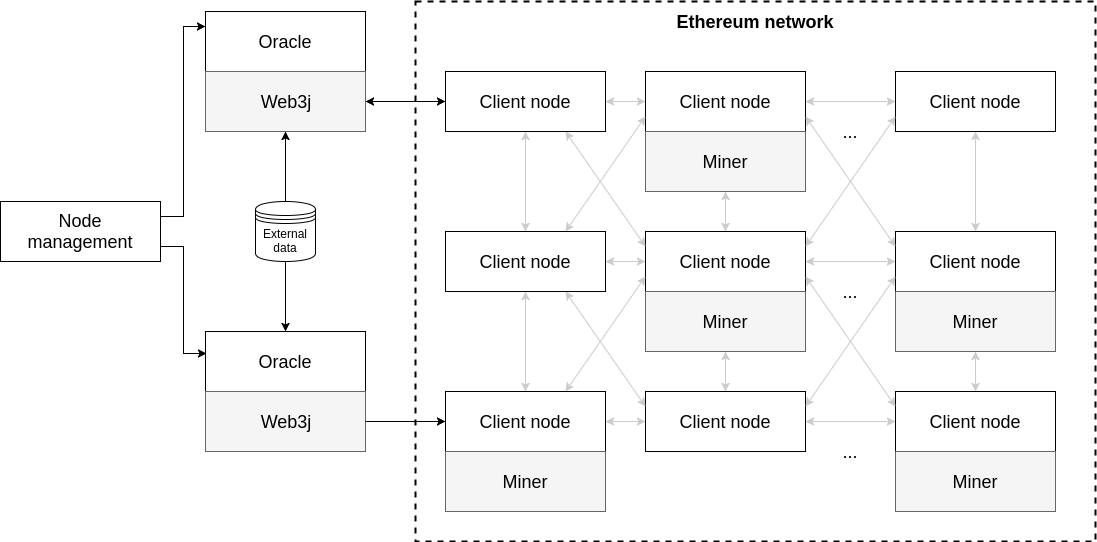
\includegraphics[width=0.7\textwidth]{blockchain-microservice-architecture.png}
  \caption{Blockchain Service Architecture}
  \label{fig:architecture}
\end{figure*}

\begin{figure*}
  \centering
  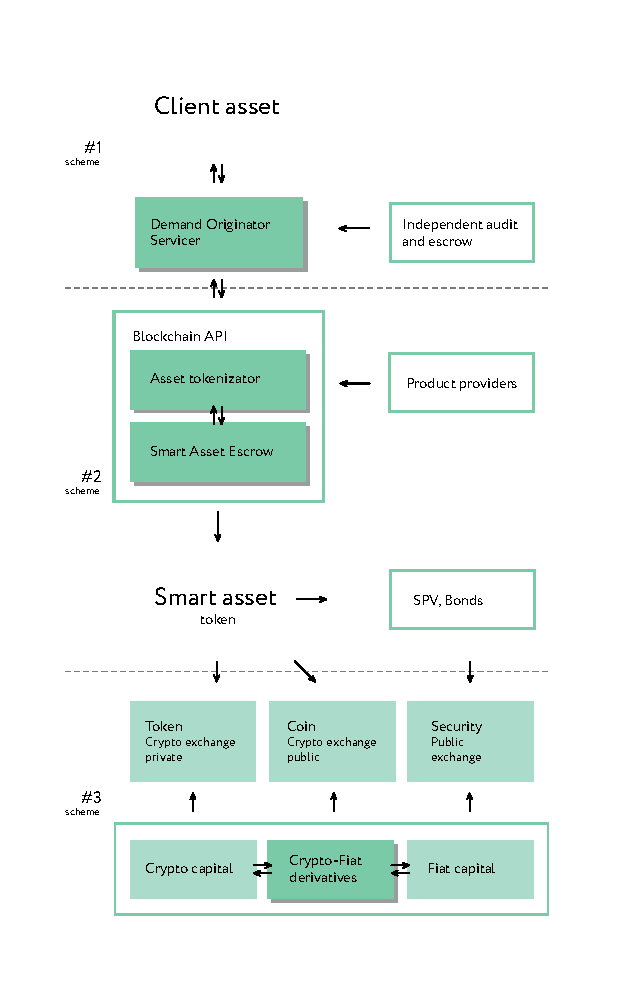
\includegraphics[width=\columnwidth]{asset-tokenization.eps}
  \caption{Asset Tokenization}
  \label{fig:tokenization}
\end{figure*}


\subsection{Blockchain Serviсe Architecture (BlockSA) Difficulty Tuning}

\subsection{What is Blockchain Serviсe Architecture (BlockSA)}

\subsection{Liquidity Theory Through the Prizm of Tokenization}

\subsection{Market Making Mathematical Models for Smart Asset}

\begin{table}[h]
    \caption{Key players}
    \label{tab:players}\centering
    \begin{tabularx}{\textwidth}{|X|c|}
        \hline
            \thead{30-Day Liquidity-Making \\ Buy/Sell Ratio} & \thead{Maker Discount (bps)} \\
        \hline
            \makecell{Worse than 35/65 (or 65/35)} & \makecell{0} \\
            \makecell{35/65 (or 65/35) or better} & \makecell{0} \\
            \makecell{40/60 (or 60/40) or better} & \makecell{10} \\
            \makecell{45/55 (or 55/45) or better} & \makecell{15} \\
        \hline
    \end{tabularx}
\end{table}

\begin{table}[h]
    \caption{Roles}
    \label{tab:roles}\centering
    \begin{tabularx}{14cm}{|l|X|}
        \hline
            \thead{Player} & \thead{Role} \\
        \hline
            Traders & Make buy/sell orders \\
            Market makers (speciaists) & Display public buy \& sell quotations for a guaranteed number of security/good to traders and fulfill orders from traders at these quotations \\
            Dealers & Buy and sell security/good from traders but do not disclose quotes publicly \\
            Brokers & Execute orders on behalf of its clients \\
        \hline
    \end{tabularx}
\end{table}

We use the following notation in our formulas:
\begin{itemize}
    \item Trading volume disccount: $D_{Trading Volume}$
    \item Buy/Sell Ratio Discount: $D_{Buy\over{Sell}}$
    \item Total Maker trading volume $V_{Maker}$
    \item Total Taker trading volume $V_{Taker}$
\end{itemize}

Maker:
\begin{equation}
  f_{Maker} = \Big(25-D_{Trading Volume} - D_{Buy \over{Sell}}\Big) \times V_{Maker}
\end{equation}

Taker:
\begin{equation}
    f_{Taker} = \Big(25-D_{Trading Volume}\Big) \times V_{Taker},
\end{equation}

\begin{equation*}
    \text{where}~D_{Trading Volume} =
    \begin{cases} 
        0 & \text{if } V_{Taker} < 10~000~BKX \\
        10 & \text{if } V_{Taker} \geq 10~000~BKX
   \end{cases}
\end{equation*}

\begin{equation}
    f_{Total} = f_{Maker} - f_{Taker}
\end{equation}

\end{multicols}

\newpage
\appendix

\section{Terminology}
\begin{description}
\item[Blockchain]~--- is a continuously growing list of records, called \textit{blocks}, which are linked and secured using cryptography \cite{bitcoinComprehensive2016} \cite{wikipediaBlockchain}.
\item[Tokenization]~--- process of converting rights into digital token to be circulated onver blockchain with low transactional fees. Tokenization is a blockchain equivalent of securitization.
\end{description}

\printbibliography

\end{document}
